\newpage
\section{Email}
\subsection{Introduction}
Email is an example of an application that works on the different layers. It's \textbf{asynchronous}, \textbf{decentralized} (to improve \textit{scaling}), \textbf{client-server} and based on simple ASCII text.
\subsubsection{Motivation}
Email was the first \textit{killer application}. It started in the 1980's with a simple terminal interface, evolving in the 1990's with the \textit{web-mail} and then \textit{mobile email}. Today social network are trying to swallow the email concept.
\subsection{Architecture}
There are two actors involved:
\begin{itemize}
	\item \textbf{User Agent}, with email clients. Runs on the computer of the user and is intermittently on. E.g. Thunderbird or Outlook
	\item \textbf{Message Transfer Agent}: the email servers. They run on a remote machine and stores and forwards on behalf of the User Agents. It's always on
\end{itemize}

\begin{center}
	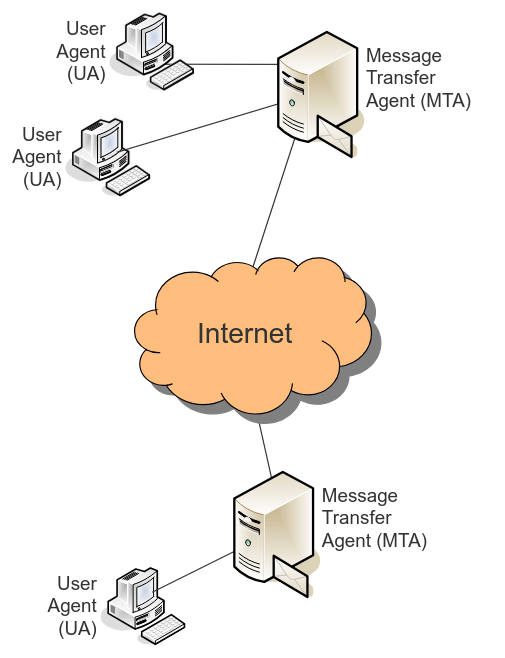
\includegraphics[scale=0.3]{email.png}
\end{center}

\subsection{Message}
Message are viewed as having an \textbf{envelope}, the fundamental part for the delivery, and a \textbf{content}. The latter contains a \textbf{header} with a certain coding and a \textbf{body} consisting of simple characters.

\subsubsection{Envelope}
The envelope is created by the \textbf{MTA} or the \textbf{MSA} and includes all the information for transporting the message. Some information are redundant with the header (like the sending and receiving address) but there are some differences, like when you send a Blind Carbon Copy message.

\begin{note}
	You can't know if the sender is correct. This can be used for evil purposes. The only way to avoid that is by encrypting or signing the email.
\end{note}

\newpage
\subsubsection{Content}
\paragraph{Header} It contains characters with the following syntax:
\begin{lstlisting}
	<key>:<value>
\end{lstlisting}
\paragraph{Body} It's the content of the email. It's separated from the header by a blank line.

Since originally the content could only contain $7bit$ ASCII, \textbf{Multipurpose Internet Mail Extensions} was invented to extend the classical format. It adds additional headers, content types and sub-types:
\begin{itemize}
	\item \textbf{MIME-version}
	\item \textbf{content-description}: string that describes the content of the message
	\item \textbf{content-id}: identifier for the content
	\item \textbf{content-transfer-encoding}: selected coding for the content (BASE64, ASCII)
	\item \textbf{content-type}: specifies the type of the body in the format \textit{type/subtype}, e.g. text, image, audio, video, etc..
\end{itemize}

\subsection{Protocols}
\subsubsection{SMTP}
Simple Mail Transport Protocol delivers the mail to the final inbox. It can't ensure that the message arrives to the final user because it expects the receiver to be always online.\\
It uses \textbf{reliable data transfer} based on TCP on port $25$ and it's \textit{best effort}. It provides \textbf{little security}: no encryption, optional authentication on port $587$ to reach MSA but nothing between MTAs.\\
The protocol follows these steps:
\begin{enumerate}
	\item \textbf{Write} an email, the client formats it and sends it to it's own mail server
	\item The mail server sets up a connection with the receiver's server and \textbf{sends} a copy of the email
	\item The \textbf{receiver}'s server creates the header of the email and places the message in the inbox
\end{enumerate}

\paragraph{Graylisting} A first attempt to block spam. If a combination of IP address of the sender, their email and the receiver's one is seen for the first time, the message is discarded and an error is returned. From the second time on, the message goes through. This is based on the idea that scammers won't send the email twice.

\subsubsection{POP3}
This protocol pulls emails from the server over a connection on port $110$. It's text based and allows basic functionalities such as \textit{logging}, \textit{copying locally} and \textit{deleting} from the server.\\
It works in two phases:
\begin{enumerate}
	\item \textbf{Authorization} phase: \textit{user}name and \textit{pass}word for authentication, either successful or not
	\item \textbf{Transaction} phase: a \textit{list} of the messages and their sizes is provided, then via \textit{retr} its possible to retrieve a message using the number of the list and with \textit{dele} to delete an email.
\end{enumerate}

\begin{note}
	POP3 is heavily limited due to problems with multiple users handling and always-on connections.
\end{note}
\subsubsection{IMAP}
This protocol works on port $143$. In this case the emails remains on the server and may be cached by the client. All the actions are performed on the server. Ideal when you need to access it from different locations.

\subsubsection{HTTP}
The \textbf{webmail} allows the user to interact with emails via WEB. E.g. Gmail or Outlook.